\subsection{Redes neuronales}

A continuación se muestran los resultados de todos los modelos con las distintas ventans que se han entrenado para estudiar como se comporta. Todos los modelos tienen los mismo hiperparámetros que se han explicado en la sección \ref{models}. A continuación, se puede ver una tabla con todos los resultados obtenidos. Las columnas representan los modelos usados, los cuales todos tienen las métricas obtenidas tanto para el \textit{dataset} de \textit{validation} como el \textit{dataset} de \textit{testing}. Las filas están dividas tanto por las métricas usadas como por el tamaño de ventana para cada modelo. En total se han desarrollado $60$ modelos ($15$ tamaños de ventanas distintos por 4 modelos de redes neuronales):


\begin{longtable}{ll|rr|rr|rr|rr}
\toprule
      &          & \multicolumn{2}{l}{Dense} & \multicolumn{2}{l}{RNN} & \multicolumn{2}{l}{LSTM} & \multicolumn{2}{l}{AR} \\
      &          & val & test & val & test & val & test & val\_ar & test\_ar \\
\midrule
\multirow{15}{*}{HUBER} & (3, 1) &     0.344 &      0.380 &   0.334 &    0.374 &    0.474 &     0.508 &  0.290 &   0.321 \\
      & (5, 1) &     0.375 &      0.411 &   0.347 &    0.388 &    0.476 &     0.510 &  0.296 &   0.330 \\
      & (8, 1) &     0.410 &      0.445 &   0.352 &    0.389 &    0.477 &     0.512 &  0.291 &   0.324 \\
      & (8, 3) &     0.348 &      0.380 &   0.331 &    0.369 &    0.293 &     0.329 &  0.295 &   0.331 \\
      & (8, 5) &     0.373 &      0.411 &   0.346 &    0.385 &    0.301 &     0.342 &  0.303 &   0.342 \\
      & (12, 1) &     0.435 &      0.472 &   0.378 &    0.418 &    0.472 &     0.506 &  0.288 &   0.320 \\
      & (12, 3) &     0.344 &      0.379 &   0.334 &    0.370 &    0.294 &     0.330 &  0.302 &   0.338 \\
      & (12, 5) &     0.371 &      0.409 &   0.346 &    0.386 &    0.303 &     0.340 &  0.307 &   0.344 \\
      & (24, 1) &     0.460 &      0.495 &   0.434 &    0.474 &    0.472 &     0.507 &  0.290 &   0.323 \\
      & (24, 3) &     0.353 &      0.386 &   0.332 &    0.370 &    0.295 &     0.331 &  0.300 &   0.335 \\
      & (24, 5) &     0.363 &      0.401 &   0.347 &    0.386 &    0.301 &     0.341 &  0.311 &   0.348 \\
      & (36, 8) &     0.355 &      0.399 &   0.358 &    0.397 &    0.299 &     0.338 &  0.317 &   0.358 \\
      & (36, 12) &     0.362 &      0.403 &   0.373 &    0.409 &    0.306 &     0.348 &  0.335 &   0.385 \\
      & (48, 12) &     0.367 &      0.408 &   0.370 &    0.409 &    0.306 &     0.347 &  0.327 &   0.369 \\
      & (48, 24) &     0.374 &      0.414 &   0.385 &    0.423 &    0.311 &     0.353 &  0.337 &   0.374 \\
\hline \multirow{15}{*}{MSLE}  & (3, 1) &     0.136 &      0.154 &   0.130 &    0.149 &    0.235 &     0.253 &  0.115 &   0.131 \\
      & (5, 1) &     0.153 &      0.171 &   0.140 &    0.160 &    0.240 &     0.258 &  0.117 &   0.134 \\
      & (8, 1) &     0.177 &      0.195 &   0.143 &    0.162 &    0.242 &     0.261 &  0.115 &   0.131 \\
      & (8, 3) &     0.134 &      0.151 &   0.129 &    0.148 &    0.114 &     0.131 &  0.118 &   0.135 \\
      & (8, 5) &     0.149 &      0.170 &   0.136 &    0.156 &    0.117 &     0.135 &  0.123 &   0.142 \\
      & (12, 1) &     0.198 &      0.217 &   0.157 &    0.177 &    0.233 &     0.251 &  0.117 &   0.132 \\
      & (12, 3) &     0.132 &      0.150 &   0.129 &    0.147 &    0.114 &     0.131 &  0.123 &   0.140 \\
      & (12, 5) &     0.148 &      0.169 &   0.136 &    0.157 &    0.118 &     0.135 &  0.124 &   0.142 \\
      & (24, 1) &     0.217 &      0.235 &   0.194 &    0.217 &    0.234 &     0.252 &  0.118 &   0.134 \\
      & (24, 3) &     0.137 &      0.154 &   0.130 &    0.149 &    0.115 &     0.132 &  0.122 &   0.139 \\
      & (24, 5) &     0.144 &      0.164 &   0.138 &    0.157 &    0.117 &     0.136 &  0.129 &   0.148 \\
      & (36, 8) &     0.144 &      0.167 &   0.142 &    0.163 &    0.119 &     0.138 &  0.128 &   0.148 \\
      & (36, 12) &     0.148 &      0.169 &   0.148 &    0.166 &    0.121 &     0.141 &  0.138 &   0.162 \\
      & (48, 12) &     0.150 &      0.172 &   0.150 &    0.170 &    0.121 &     0.141 &  0.135 &   0.156 \\
      & (48, 24) &     0.154 &      0.175 &   0.155 &    0.175 &    0.122 &     0.142 &  0.139 &   0.158 \\
\hline 
\multirow{15}{*}{MSE} & (3, 1) &     2.518 &      2.802 &   2.513 &    2.831 &    4.958 &     5.302 &  1.623 &   1.793 \\
      & (5, 1) &     3.228 &      3.526 &   2.678 &    3.022 &    5.017 &     5.375 &  1.684 &   1.899 \\
      & (8, 1) &     3.885 &      4.144 &   2.755 &    3.018 &    5.028 &     5.392 &  1.622 &   1.826 \\
      & (8, 3) &     2.792 &      3.012 &   2.454 &    2.736 &    1.740 &     2.025 &  1.692 &   1.976 \\
      & (8, 5) &     3.185 &      3.550 &   2.730 &    3.031 &    1.890 &     2.284 &  1.839 &   2.155 \\
      & (12, 1) &     4.278 &      4.593 &   3.237 &    3.514 &    5.017 &     5.358 &  1.582 &   1.785 \\
      & (12, 3) &     2.746 &      3.017 &   2.557 &    2.830 &    1.784 &     2.081 &  1.810 &   2.052 \\
      & (12, 5) &     3.171 &      3.510 &   2.692 &    2.998 &    1.929 &     2.240 &  1.895 &   2.187 \\
      & (24, 1) &     4.653 &      4.974 &   4.393 &    4.749 &    5.032 &     5.389 &  1.604 &   1.818 \\
      & (24, 3) &     2.831 &      3.069 &   2.448 &    2.724 &    1.751 &     2.038 &  1.749 &   2.002 \\
      & (24, 5) &     2.990 &      3.330 &   2.701 &    2.980 &    1.872 &     2.222 &  2.122 &   2.403 \\
      & (36, 8) &     2.724 &      3.146 &   2.928 &    3.220 &    1.743 &     2.111 &  2.014 &   2.404 \\
      & (36, 12) &     2.880 &      3.225 &   3.210 &    3.475 &    1.870 &     2.272 &  2.327 &   2.842 \\
      & (48, 12) &     2.965 &      3.333 &   3.098 &    3.372 &    1.855 &     2.246 &  2.093 &   2.476 \\
      & (48, 24) &     3.081 &      3.431 &   3.377 &    3.653 &    1.950 &     2.350 &  2.357 &   2.649 \\
\hline \multirow{15}{*}{MAE} & (3, 1) &     0.508 &      0.550 &   0.519 &    0.565 &    0.699 &     0.738 &  0.468 &   0.504 \\
      & (5, 1) &     0.546 &      0.587 &   0.543 &    0.592 &    0.674 &     0.713 &  0.475 &   0.515 \\
      & (8, 1) &     0.594 &      0.636 &   0.542 &    0.586 &    0.672 &     0.711 &  0.469 &   0.508 \\
      & (8, 3) &     0.524 &      0.563 &   0.521 &    0.565 &    0.469 &     0.512 &  0.455 &   0.498 \\
      & (8, 5) &     0.546 &      0.591 &   0.535 &    0.581 &    0.477 &     0.524 &  0.461 &   0.506 \\
      & (12, 1) &     0.642 &      0.685 &   0.561 &    0.609 &    0.702 &     0.741 &  0.444 &   0.481 \\
      & (12, 3) &     0.519 &      0.560 &   0.520 &    0.562 &    0.469 &     0.512 &  0.458 &   0.501 \\
      & (12, 5) &     0.545 &      0.590 &   0.537 &    0.583 &    0.478 &     0.522 &  0.463 &   0.506 \\
      & (24, 1) &     0.677 &      0.718 &   0.629 &    0.674 &    0.704 &     0.743 &  0.446 &   0.485 \\
      & (24, 3) &     0.526 &      0.564 &   0.522 &    0.567 &    0.473 &     0.515 &  0.453 &   0.494 \\
      & (24, 5) &     0.536 &      0.580 &   0.539 &    0.585 &    0.477 &     0.523 &  0.467 &   0.511 \\
      & (36, 8) &     0.548 &      0.599 &   0.551 &    0.598 &    0.477 &     0.523 &  0.475 &   0.523 \\
      & (36, 12) &     0.556 &      0.604 &   0.562 &    0.606 &    0.485 &     0.534 &  0.488 &   0.545 \\
      & (48, 12) &     0.559 &      0.608 &   0.571 &    0.617 &    0.485 &     0.533 &  0.479 &   0.530 \\
      & (48, 24) &     0.570 &      0.618 &   0.582 &    0.626 &    0.491 &     0.539 &  0.490 &   0.534 \\
\hline \multirow{15}{*}{RMSE} & (3, 1) &     1.587 &      1.674 &   1.585 &    1.683 &    2.225 &     2.303 &  1.273 &   1.339 \\
      & (5, 1) &     1.797 &      1.877 &   1.637 &    1.739 &    2.241 &     2.319 &  1.297 &   1.378 \\
      & (8, 1) &     1.972 &      2.037 &   1.660 &    1.738 &    2.244 &     2.322 &  1.274 &   1.351 \\
      & (8, 3) &     1.671 &      1.735 &   1.567 &    1.655 &    1.318 &     1.424 &  1.301 &   1.406 \\
      & (8, 5) &     1.785 &      1.885 &   1.653 &    1.740 &    1.375 &     1.511 &  1.356 &   1.468 \\
      & (12, 1) &     2.070 &      2.143 &   1.796 &    1.876 &    2.238 &     2.317 &  1.258 &   1.337 \\
      & (12, 3) &     1.659 &      1.738 &   1.598 &    1.679 &    1.336 &     1.441 &  1.346 &   1.434 \\
      & (12, 5) &     1.782 &      1.876 &   1.642 &    1.732 &    1.389 &     1.497 &  1.377 &   1.478 \\
      & (24, 1) &     2.157 &      2.230 &   2.096 &    2.179 &    2.243 &     2.321 &  1.266 &   1.348 \\
      & (24, 3) &     1.682 &      1.752 &   1.565 &    1.651 &    1.323 &     1.428 &  1.323 &   1.415 \\
      & (24, 5) &     1.729 &      1.825 &   1.643 &    1.726 &    1.368 &     1.491 &  1.457 &   1.550 \\
      & (36, 8) &     1.649 &      1.772 &   1.712 &    1.795 &    1.320 &     1.453 &  1.419 &   1.550 \\
      & (36, 12) &     1.697 &      1.798 &   1.792 &    1.865 &    1.366 &     1.508 &  1.526 &   1.685 \\
      & (48, 12) &     1.722 &      1.826 &   1.760 &    1.836 &    1.362 &     1.499 &  1.447 &   1.574 \\
      & (48, 24) &     1.755 &      1.853 &   1.837 &    1.911 &    1.397 &     1.533 &  1.535 &   1.627 \\
\hline \multirow{15}{*}{RMSLE} & (3, 1) &     0.367 &      0.391 &   0.360 &    0.385 &    0.484 &     0.501 &  0.339 &   0.360 \\
      & (5, 1) &     0.390 &      0.413 &   0.373 &    0.399 &    0.488 &     0.506 &  0.342 &   0.365 \\
      & (8, 1) &     0.420 &      0.440 &   0.377 &    0.401 &    0.490 &     0.509 &  0.339 &   0.361 \\
      & (8, 3) &     0.365 &      0.388 &   0.359 &    0.384 &    0.337 &     0.362 &  0.343 &   0.367 \\
      & (8, 5) &     0.385 &      0.411 &   0.368 &    0.394 &    0.341 &     0.367 &  0.350 &   0.376 \\
      & (12, 1) &     0.444 &      0.465 &   0.395 &    0.420 &    0.481 &     0.500 &  0.341 &   0.363 \\
      & (12, 3) &     0.362 &      0.387 &   0.358 &    0.383 &    0.337 &     0.361 &  0.350 &   0.374 \\
      & (12, 5) &     0.384 &      0.410 &   0.369 &    0.395 &    0.342 &     0.367 &  0.351 &   0.376 \\
      & (24, 1) &     0.464 &      0.484 &   0.439 &    0.464 &    0.482 &     0.501 &  0.343 &   0.366 \\
      & (24, 3) &     0.369 &      0.392 &   0.360 &    0.385 &    0.339 &     0.363 &  0.349 &   0.372 \\
      & (24, 5) &     0.378 &      0.404 &   0.370 &    0.396 &    0.342 &     0.368 &  0.359 &   0.384 \\
      & (36, 8) &     0.379 &      0.408 &   0.377 &    0.403 &    0.344 &     0.370 &  0.357 &   0.385 \\
      & (36, 12) &     0.384 &      0.411 &   0.384 &    0.407 &    0.347 &     0.375 &  0.371 &   0.402 \\
      & (48, 12) &     0.387 &      0.414 &   0.387 &    0.412 &    0.347 &     0.375 &  0.367 &   0.395 \\
      & (48, 24) &     0.392 &      0.418 &   0.394 &    0.418 &    0.350 &     0.377 &  0.372 &   0.397 \\
\bottomrule
\end{longtable}

También se han desarrollado gráficas para poder visualizar las métricas más fácilmente usando usando el dataset de \textit{testing}. En todas las gráficas hay una línea horizontal que representa la métrica obtenida por el modelo base:



\begin{figure}[H]
    \centering
    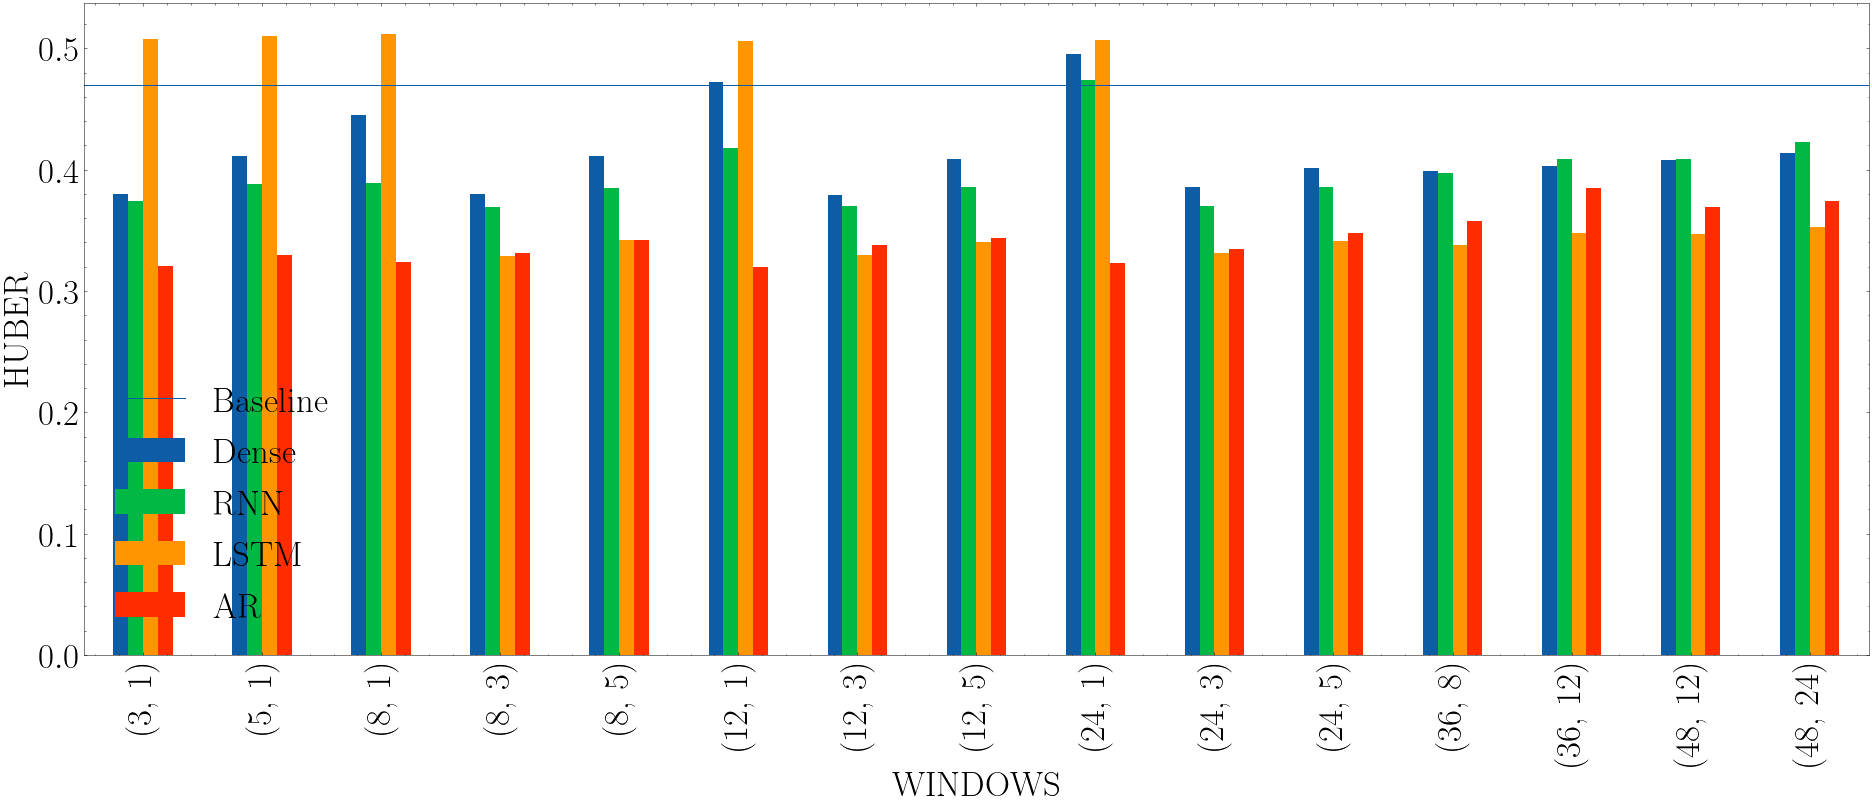
\includegraphics[width=15cm]{images/solution/metrics/HUBER.png}
    \caption{Resultados usando pérdida de Huber}
\end{figure}

\begin{figure}[H]
    \centering
    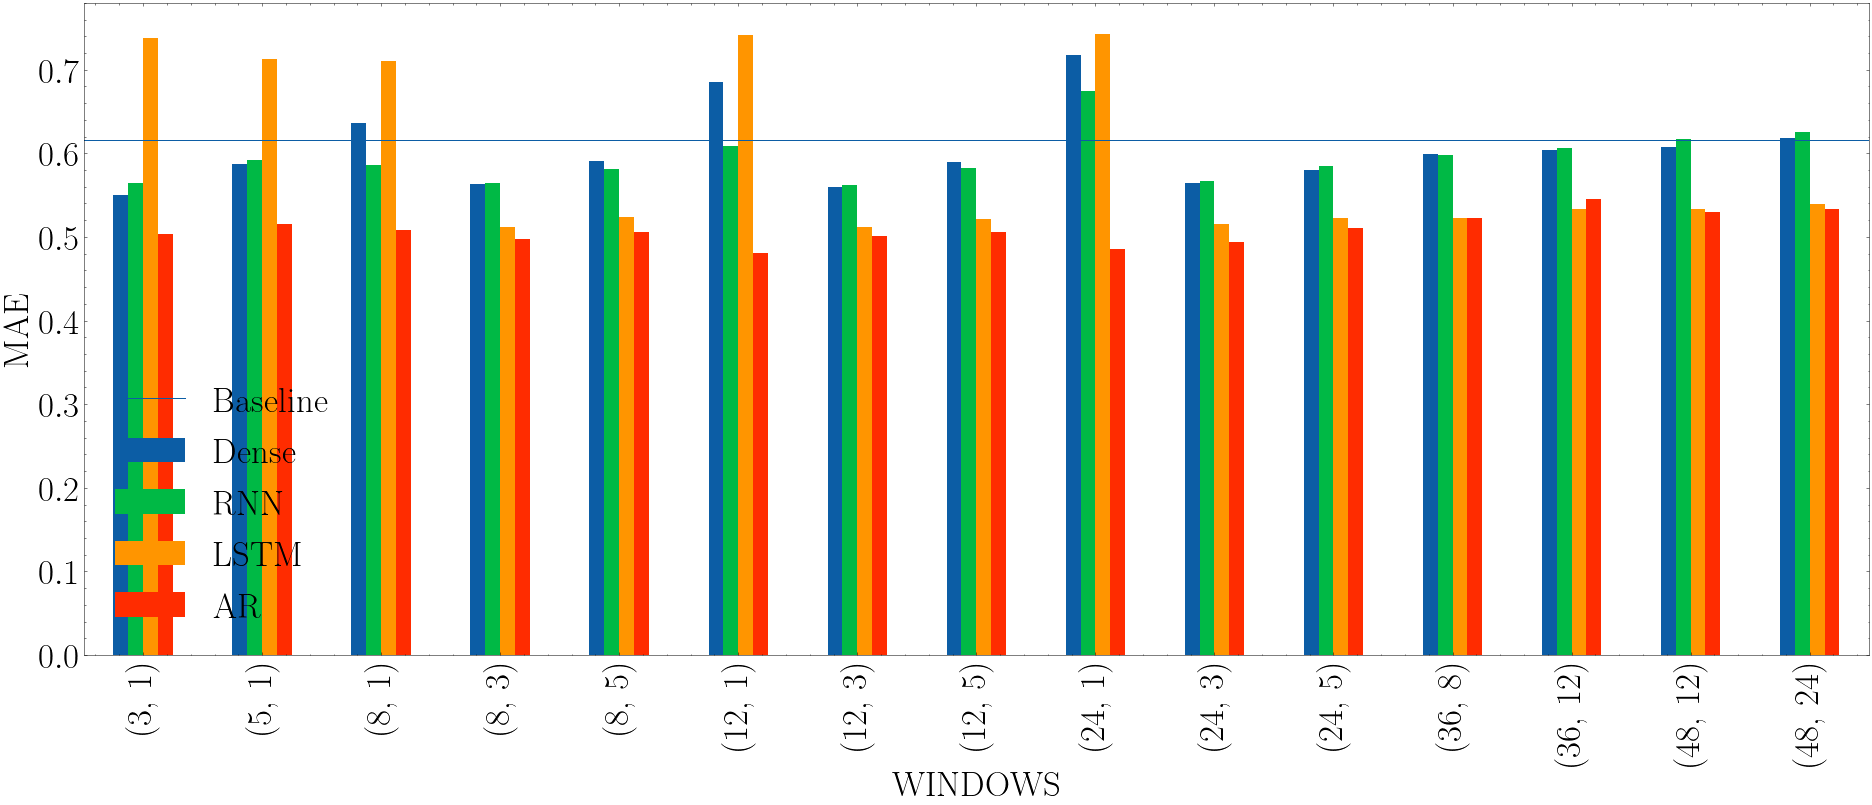
\includegraphics[width=15cm]{images/solution/metrics/MAE.png}
    \caption{Métricas usando MAE}
\end{figure}

\begin{figure}[H]
    \centering
    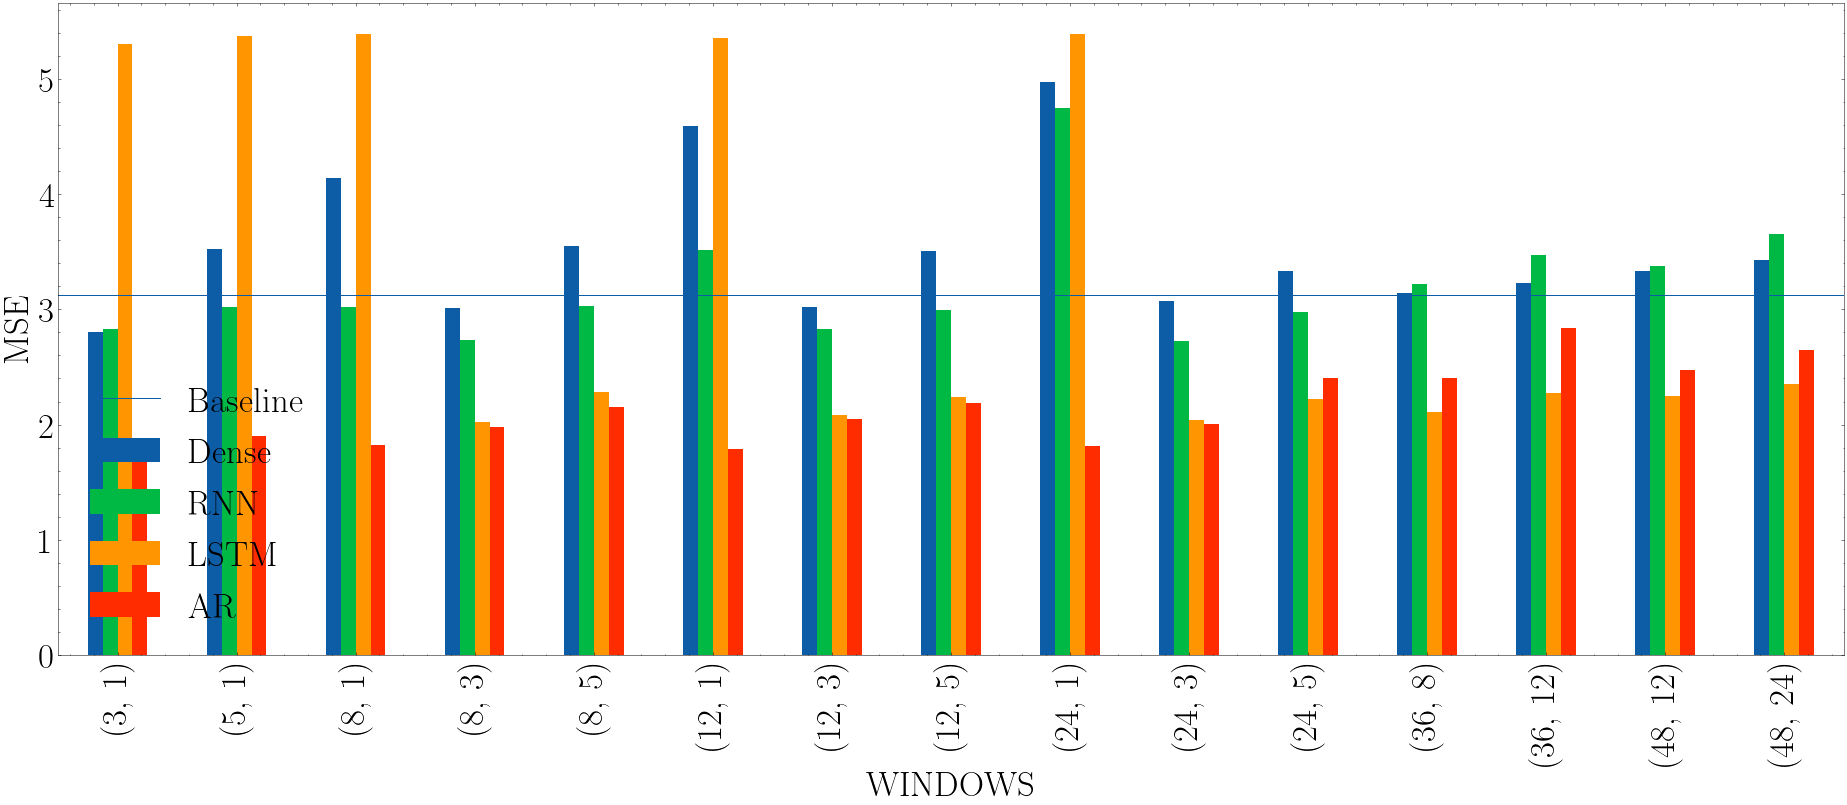
\includegraphics[width=15cm]{images/solution/metrics/MSE.png}
    \caption{Métricas usando MSE}
\end{figure}

\begin{figure}[H]
    \centering
    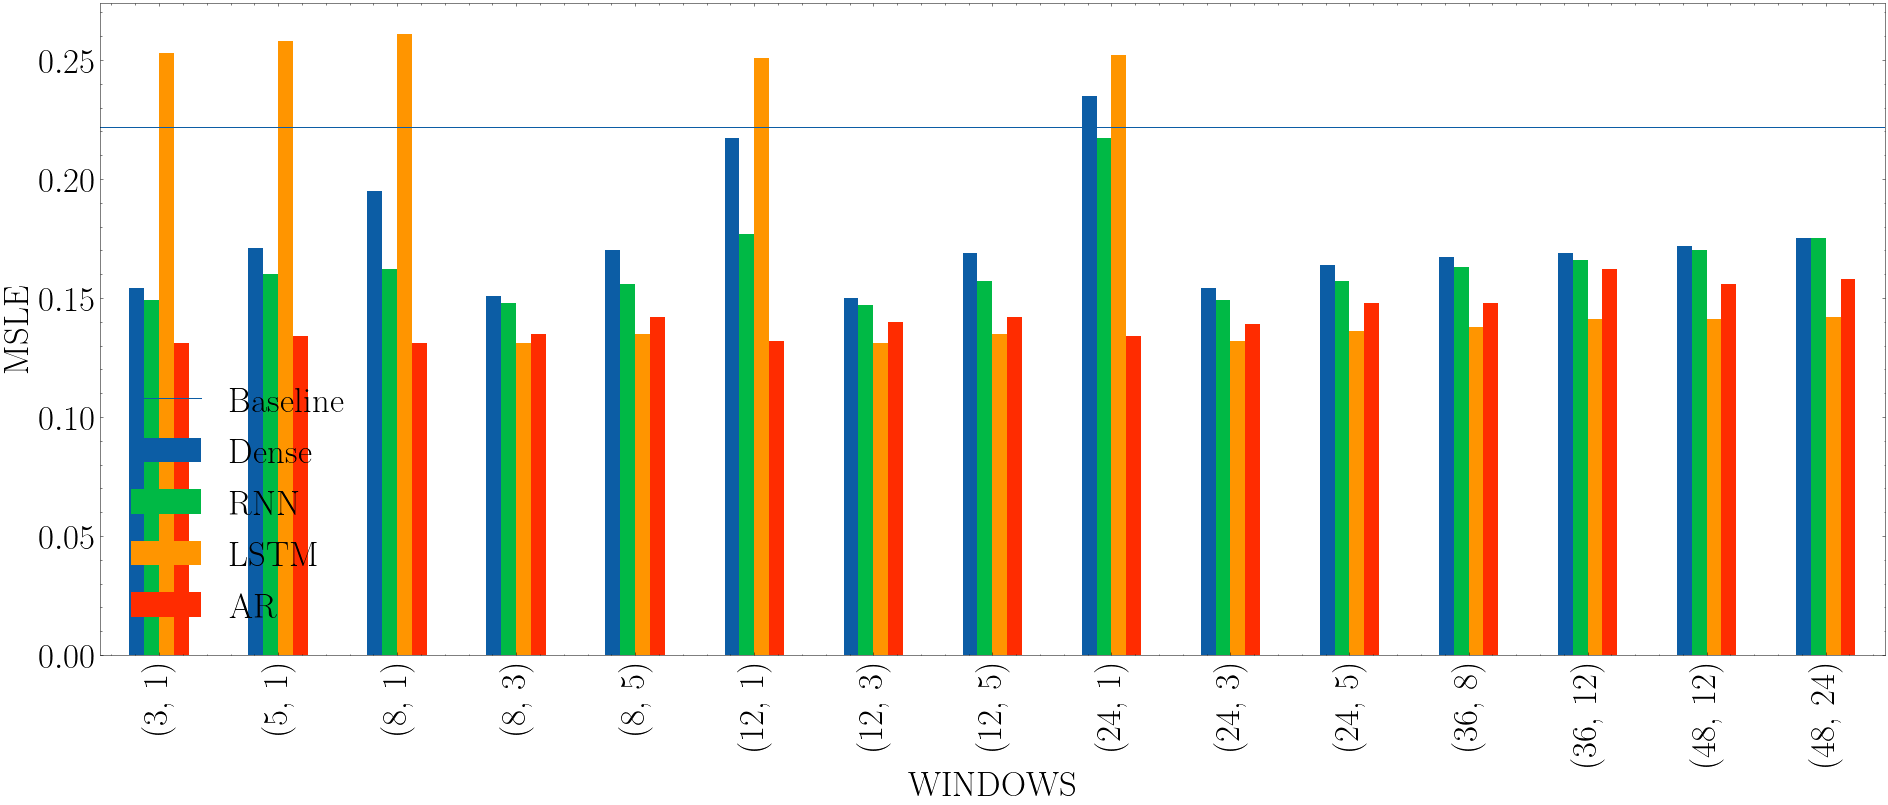
\includegraphics[width=15cm]{images/solution/metrics/MSLE.png}
    \caption{Métricas usando MSLE}
\end{figure}

\begin{figure}[H]
    \centering
    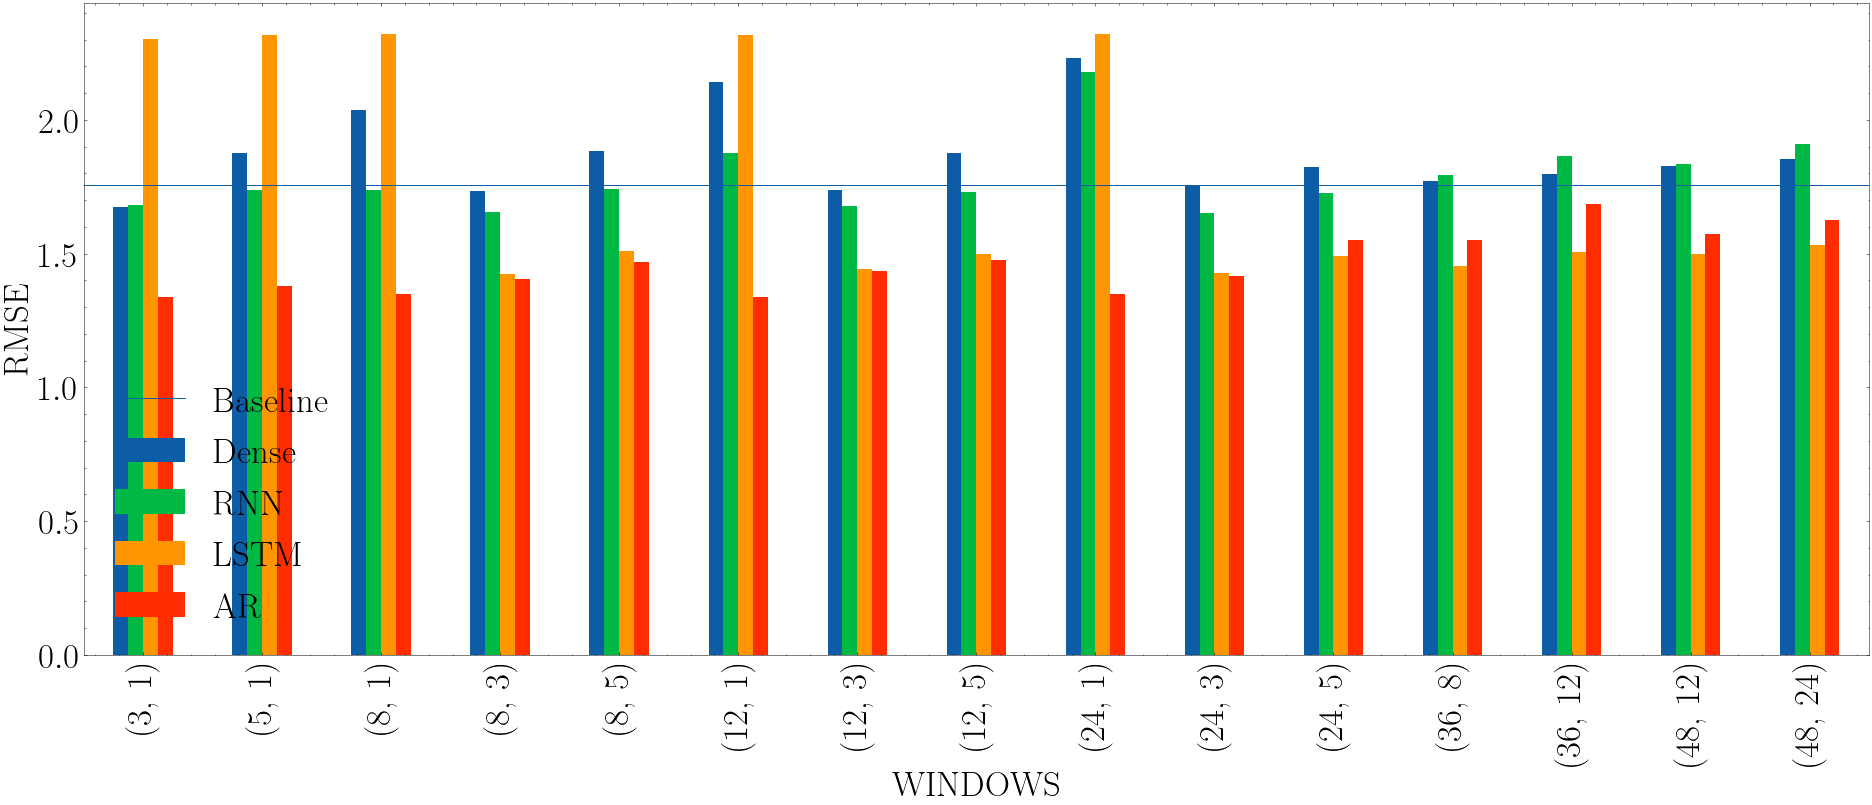
\includegraphics[width=15cm]{images/solution/metrics/RMSE.png}
    \caption{Métricas usando RMSE}
\end{figure}

\begin{figure}[H]
    \centering
\end{figure}